%%%%%%%%%%%%%%%%%%%%%%% file template.tex %%%%%%%%%%%%%%%%%%%%%%%%%
%
% This is a general template file for the LaTeX package SVJour3
% for Springer journals.          Springer Heidelberg 2010/09/16
%
% Copy it to a new file with a new name and use it as the basis
% for your article. Delete % signs as needed.
%
% This template includes a few options for different layouts and
% content for various journals. Please consult a previous issue of
% your journal as needed.
%
%%%%%%%%%%%%%%%%%%%%%%%%%%%%%%%%%%%%%%%%%%%%%%%%%%%%%%%%%%%%%%%%%%%
%
% First comes an example EPS file -- just ignore it and
% proceed on the \documentclass line
% your LaTeX will extract the file if required
%\begin{filecontents*}{example.eps}
%%!PS-Adobe-3.0 EPSF-3.0
%%%BoundingBox: 19 19 221 221
%%%CreationDate: Mon Sep 29 1997
%%%Creator: programmed by hand (JK)
%%%EndComments
%gsave
%newpath
%  20 20 moveto
%  20 220 lineto
%  220 220 lineto
%  220 20 lineto
%closepath
%2 setlinewidth
%gsave
%  .4 setgray fill
%grestore
%stroke
%grestore
%\end{filecontents*}
%%
%\RequirePackage{fix-cm}
%
%\documentclass{svjour3}                     % onecolumn (standard format)
%\documentclass[smallcondensed]{svjour3}     % onecolumn (ditto)
%%%% \documentclass[smallextended]{svjour3}       % onecolumn (second format)
\documentclass[twocolumn]{svjour3}          % twocolumn
%
\smartqed  % flush right qed marks, e.g. at end of proof
%
\usepackage{graphicx}
\usepackage{multirow}
\usepackage[misc,geometry]{ifsym}
\usepackage{url}
\usepackage[dvips]{hyperref}
\usepackage{cite}
\usepackage{fix-cm}
\usepackage{balance}
\usepackage{array}

%
% \usepackage{mathptmx}      % use Times fonts if available on your TeX system
%
% insert here the call for the packages your document requires
%\usepackage{latexsym}
% etc.
%
% please place your own definitions here and don't use \def but
% \newcommand{}{}
%
% Insert the name of "your journal" with
%\journalname{myjournal}
%

\newcommand{\Lukas}{Luk{\' a\v s} {\em et  al.}}

\begin{document}

%\title{Source Camera Identification in Real Practice: Experimentations with Online Social Networks\thanks{The project is a joint work with the CNCPO (\textsl{Centro Nazionale per il Contrasto 
%della Pedopornografia Online}), part of the ``Dipartimento della Pubblica Sicurezza'' within 
%the Italian Ministry of Interior.}
%}

\title{Experimentations with Source Camera Identification and Online Social Networks
\thanks{The project is a joint work with the CNCPO (\textsl{Centro Nazionale per il Contrasto 
della Pedopornografia Online}), part of the ``Dipartimento della Pubblica Sicurezza'' within 
the Italian Ministry of Interior.}
\thanks{A preliminary version of this paper appeared in the International Workshop on Cloud, Wireless and e-Commerce Security (CWECS 2010) held in Fukuoka, November 4-6, 2010.}
}

% \subtitle{Do you have a subtitle?\\ If so, write it here}

%\titlerunning{Short form of title}        % if too long for running head

\author{ {Umberto Ferraro Petrillo} \and {Aniello Castiglione} \and {Giuseppe Cattaneo} \and {Maurizio Cembalo} }

%\authorrunning{Short form of author list} % if too long for running head

\institute{Umberto Ferraro Petrillo (\Letter) \at
              Dipartimento di Scienze Statistiche\\
              Universit\`a degli Studi di Roma ``\textit{La Sapienza}''\\
              P.le Aldo Moro 5, I-00185 Rome, Italy\\
              \email{umberto.ferraro@uniroma1.it }
              \and
              Aniello Castiglione \and Giuseppe Cattaneo \and \\ Maurizio Cembalo \at
              Dipartimento di Informatica ``\textit{R.M. Capocelli}'' \\
              Universit\`{a} degli Studi di Salerno\\
              Via Ponte don Melillo, I-84084 Fisciano (SA), Italy\\
              Tel.: +39-089-969594, Fax: +39-089-969600\\
              \email{castiglione@\{ieee,acm\}.org, cattaneo@dia.unisa.it, maucem@dia.unisa.it}           %  \\
%             \emph{Present address:} of F. Author  %  if needed
}

\date{Received: date / Accepted: date}
% The correct dates will be entered by the editor


\maketitle

\begin{abstract}
In this paper is presented an extended experimental evaluation of one of the most effective source camera identification techniques proposed so far, by Luk{\' a\v s} {\em et  al.}. This method uses the characteristic noise left by the sensor on a digital picture as a fingerprint in order to identify the source camera used to take the picture. 
The aim of the experiments is to assess the effectiveness of this technique when used with pictures that were previously modified using several common image-processing functions coming with photo-editing tools. Moreover, the technique is applied to photos passed through Online Social Networks or Online Photo Sharing websites, without any ``human'' explicit modification but only elaborated by such Web 2.0 tools.

The results confirm that, in several cases, the method by \Lukas\ is resilient to the modifications introduced by the considered image-processing functions. However, in the experiments it has been possible to identify several cases where the quality of the identification process deteriorated because of the noise introduced by the image-processing. In addition, when dealing with Online Social Networks and Online Photo Sharing services, it has been noted that some of them process and modify the uploaded pictures. These modifications make ineffective, in many cases, the method by \Lukas.\

\keywords{Online Social Networks \and Online Photo Sharing \and Image Forensics \and Digital Forensics \and Digital Camera Identification \and Digital Camera Model Identification \and Digital Investigations.}
% \PACS{PACS code1 \and PACS code2 \and more}
% \subclass{MSC code1 \and MSC code2 \and more}
\end{abstract}

% This section will introduce the general problem of digital camera
% identification and its applications to the field of digital forensic. 
% Moreover, we will discuss about existing contributions in the
% following terms.

% Several approaches have been proposed so far to this end. Many of
% these approaches have also been experimented using large sets of
% digital images. 

\section{Introduction}
Nowadays, taking and sharing digital pictures is becoming a very popular activity.  This is witnessed by the explosive growth of the digital cameras market: e.g., more than one billion digital cameras have been produced and shipped in 2010~\cite{cipa}.  A consequence of this trend is that also the number of crimes involving digital pictures increases, either because pictures are part of the crime (e.g., exchanging pedopornographic pictures) or because their analysis may reveal some important clue about the author of the crime.  Image Forensics tries to help the investigators when in presence of digital photographic evidence. One of the many issues that the Image Forensics tries to deal with is the {\em source camera identification problem}, i.e., establish if a given image has been taken by a given digital camera. Many identification techniques have been proposed so far in literature. All these techniques generally work by using the sensor noise left by a digital sensor when taking a picture as a fingerprint for identifying the sensor. These studies are generally accompanied with tests proving the effectiveness of these techniques, both in terms of False Acceptance Rate (FAR) and False Rejection Rate (FRR).  

Unfortunately, most of these contributions do not take into consideration that, in practice, the images that are shared and exchanged over the Internet have often been pre-processed. Instead, it is a common practice to assume that the images to be examined are unmodified or, at most, to ignore the effects of the pre-processing.

Even without considering the case of malicious users that could intentionally process a picture in order to fool the existing identification techniques, this assumption is unrealistic for at least two reasons. The first is that, as previously mentioned, almost all current photo-managing software offers several functions for adjusting, sometimes in a ``magic'' way (see the ``I'm feeling lucky'' function
on Google Picasa~\cite{picasa}) different characteristics of a picture. The second reason can be found in the way the images are managed by some of the most important online social network (OSN) and online photo sharing (OPS) sites. These services usually make several modifications to the original photos before publishing them in order to either improve their appearance or  reduce their size.

The contribution of this paper aims to understand how one of the most prominent source camera identification techniques performs when in the presence of pre-processed images either explicit modified by a user with photo management tools or by OSNs and OPSs services without user awareness.


%In the digital era, the creation and the modification of images (as well as videos) can be carried out at a very low cost with simple editing tools which are widely and easily accessible to everyone. As a consequence, it is not possible to always consider an image or a video authentic. This simple fact may become an issue when an image or video is digital evidence in a criminal/legal investigation. 
%

\subsection{Organization of the Paper} 
In Section~\ref{sec:did} some basic definitions about the source camera identification problem are provided as well as the current literature on this topic briefly reviewed. In Section~\ref{sec:luk} details of the identification technique presented by Luk{\' a\v s} {\em et  al.} are introduced, based on the Photo-Response Non-Uniformity of both CCD~\cite{Janesick95} and CMOS sensors~\cite{Holst96}.
In Section~\ref{sec:exp_set} are explained the conditions under which the tests have been conducted, while in Section~\ref{sec:exp_ana} the results of several tests of this technique, performed on a test-sample of nearly 2500 images taken from 8 different cameras, are presented. In the tests, the performance of this technique, when applied to the identification of the cameras used to take both modified and unmodified pictures, is compared. The core part of the work is Section~\ref{exp4} where the tests aim to understand if, and how, the OSNs and OPSs services modify the pictures uploaded by a user on such websites, and which are the consequences of these modifications on the identification process. Finally, Section~\ref{sec:conc} presents some concluding remarks. 

%The source code for our software implementation and the images used in our experimentation
%are available for download at the following address ... (???)

\section{Digital Camera Identification}
\label{sec:did}

Every digital picture contains a random component of
noise as well as a deterministic component, the {\em pattern noise}, that
depends on the sensor used to shoot the picture. The pattern noise is
``very'' similar within all the pictures taken by the same sensor. 


The problem of digital camera identification concerns with the
identification of the camera that has been used to generate a digital picture, by examining the pattern noise in the picture. This technique is called {\em source camera identification} and should not be confused with the more general {\em digital camera model identification} problem, in which there is only interest in establishing which camera model has been used to take a certain picture. 


Up until now, three main approaches were proposed in literature to deal with 
the source camera identification problem. These approaches differ in the
type of pattern noise used. 

The first approach uses the {\em Photo-Response Non-Uniformity} (PRNU)
noise, i.e., the noise produced by the sensor due to the inhomogeneity of 
the silicon wafers used to build it. Luk{\' a\v s} {\em et  al.}~\cite{Lukas06} and Chen {\em et al.}~\cite{Chen08}
proposed two methods to identify the source camera based on the
PRNU. These techniques can be used to isolate and extract the noise pattern from a set of pictures taken with the same camera, using this pattern to match or not the cameras with the photos under investigation. Their results show that these methods have high detection rates.
Goljan {\em et al} in~\cite{Goljian09} used a refinement of  the method of Chen
to run a digital camera identification test on a massive
database of digital pictures downloaded from the Internet.   

The second approach uses the lens radial distortion that causes
straight lines to appear as curved lines on the output images. Choi {\em et al.} have tried this method
 in~\cite{Choi06}. They discovered that this method failed to measure
the radial distortion except when there are explicit straight lines in the picture to be processed.

The last approach relies on the \emph{Color Filter Array} (CFA) interpolation, which is a technique
used by digital cameras after a picture has been taken in order to
determine the colors of the scene. This technique produces small
non-uniform color zones that can be seen as a noise
source. Every camera has its own interpolation algorithms and produces a small degree of noise that, 
generally, changes slightly from one camera to another.
Bayram~{\em et al.} in~\cite{Bayram05} explored the CFA interpolation process to
determine the correlation structure present in each color band which
can be used for image classification. 
In this direction, Kharrazi~{\em et al.} in~\cite{Kharrazi04} and Long and 
Huang in~\cite{Long06} proposed two methods. The first method identifies a set of
image features that can be used to uniquely classify a camera model. 
The accuracy of this method decreases as the number of cameras increases. 
The second method obtains a coefficient matrix from a quadratic pixel correlation model
 where spatially periodic inter-pixel correlation follows a quadratic form. 
The results seem to suggest that these two methods work better for the problem of camera model 
identification rather than for that of source camera identification.

% The sensor of a digital camera can only capture the luminance of a scene, not its colors. This
% information is determined by the CFA interpolation technique applied
% on the picture after this has been taken. 


% the noise produced by the {\em imperfections}
% \cite{Janesick95, Holst96} existing in every digital camera sensor as
% a fingerprint for tracing back to the camera used to shoot a picture.

% In the image acquisition process there are numerous sources of
% imperfections and noise. 

% The pattern noise is made up two main
% components: the {\em fixed pattern noise} (FPN) and the {\em
%   photo-response non uniformity noise} (PRNU).  The FPN is the
% variation of the pixel response of an image sensor in the dark; under
% these conditions particular pixels of the sensor, depending on
% exposure and temperature, are susceptible to giving brighter
% intensities. The PRNU 
% properties on the sensor.

%   The
% effect of these distortions on the resulting picture may be considered
% as the fingerprint for a digital camera.


\section{The Approach by Luk{\' a\v s} {\em et  al.}}
\label{sec:luk}

% Una delle migliori tecniche in letteratura
Attention has been focused on the approach proposed by Luk{\' a\v s} {\em et  al.}
due to it being one of the most effective method, as well as inexpensive
in terms of hardware resources unlike other similar methods such as the one proposed by Goljan in~\cite{Goljian09}.

% Come funziona la tecnica
The approach by Luk{\' a\v s} {\em et  al.} works in two stages. In the first
stage, the PRNU associated with a CCD sensor is determined by
analyzing a batch of images taken with the sensor. In the second
stage, given a picture, the procedure evaluates the correlation between 
the noise in the picture and the pattern noise evaluated in the previous stage
in order to distinguish whether the picture has been taken using that CCD 
sensor or not.

The extraction of the PRNU from an image is performed by denoising the
image using  a wavelet-based algorithm. 
The denoised image is subtracted from the original image giving as output a new
image containing several components: the CCD sensor noise, the random noise 
and various contributions from the image signal.
Thus, in order to eliminate the random component of the noise,
the denoising procedure is applied to a set of images (captured by the
same camera) and the corresponding noise residues are averaged to
obtain the reference pattern of a given digital camera. 

Afterwards, to determine whether a given image is captured by a 
digital camera, the noise pattern extracted from the given image is 
correlated with the reference pattern of the camera.  If the correlation 
value exceeds a pre-determined threshold, then the image was taken 
with that camera. In order to estimate the accuracy of the method as 
well as to compute the thresholds, the Neyman-Pearson criterion was used, 
specifying a bound on the FAR.

%I loro risultati

%This method has proven to be robust, and has also been witnessed by
%the experimentation conducted by Luk{\' a\v s} {\em et  al.}.
%However, Luk{\' a\v s} {\em et  al.} did not take in account an important issue. 
%Nowadays, it is unlikely that pictures taken using a digital camera are published
%or exchanged without first applying any sort of modification or
%resizing. Indeed, the possibility of retouching photos are 
%endless due to image editing applications currently
%available. Such applications have plenty of options for improving the quality 
%of a picture or simply for reducing its size. 
%
%The question that arises is: is the technique
%proposed by Luk{\' a\v s} {\em et  al.} resilient to these modifications? 
%In the remaining part of this paper we will try to answer to this
%question by testing this classification technique over a test set of
%pictures that have been previously processed using several common
%functions such as {\em auto level adjustment} (i.e., automatically correct 
%the tonal values in a photo), {\em auto contrast} (i.e., automatically improve 
%the contrast of a photo), {\em auto color adjustment} (i.e., automatically examine 
%a picture and remaps the colors of a picture), and {\em resizing} (using three
%different types of resizing).
%

\subsection{Implementation Details}

\begin{center}
\begin{table}[hbt]
\centering
\caption{Cameras used in the tests.}
\begin{tabular}{|l |p{2.5cm} | l | l |} 
\hline
\textbf{ID} & \textbf{Model} & \textbf{Sensor} & \textbf{Image size}  \\ \hline \hline
1 & Canon EOS 400D 				& CMOS 	& 3888x2592 \\ \hline
2 & Canon EOS 1000D 				& CMOS  	& 3888x2592 \\ \hline
3 & Canon PowerShot A400 instance A 	& CCD  	& 2048x1536  \\ \hline
4 & Canon PowerShot A400 instance B 	& CCD 	& 2048x1536  \\ \hline
5 & Panasonic Lumix DMC-FZ20 		& CCD 	& 2048x1536  \\ \hline
6 & Panasonic Lumix DMC-FS5 		& CCD 	& 3648x2736  \\ \hline
7 & Kodak EasyShare CX 7530 		& CCD 	& 2560x1920  \\ \hline
8 & HP PhotoSmart E327 				& CCD 	& 2560x1920  \\ \hline
\end{tabular}\label{cameras}
\end{table}
\end{center}

The method proposed by Luk{\' a\v s} {\em et  al.} was implemented using the 
Matlab software~\cite{MatlabSITE}. This software was used due to it being 
efficient as well as providing several pre-implemented components (e.g. wavelets functions) 
which are useful in the implementation of the various identification techniques. 

Concerning the implementation, the main element of the method proposed by Luk{\' a\v s} {\em et  al.} is the PNRU filter. This filter simulates the behaviour of the Wiener filter in the wavelet domain and it has been suggested in~\cite{Mihcak99}. The Wiener filter is based on a statistical approach and aims to filter the noise of an image.

There are several families of wavelets, each one suitable for different applications, differing 
in the number of coefficients they use. In the early stages of the tests, several combinations were
tried, with the optimal choice being 4-levels and 8-levels Daubechies wavelets.
% Fridrich usa 8-tab Binomial-QMF (Also referred to as Daubechies wavelet)


\section{Experimental Settings}
\label{sec:exp_set}

The tests were organized in three phases. In the first phase, the effectiveness of the method by Luk{\' a\v s} {\em et  al.} when applied to the camera identification for unmodified digital pictures was assessed. In the second phase, the original set of pictures were initially pre-processed using several types of image-processing functions, with identification process then being repeated, using the decision thresholds established during the first test according to non pre-processed images. In the third phase, the previous tests with pre-processed images were repeated, using the decision thresholds that have been recalculated from pre-processed images.

In all the tests, seven different camera models were considered, resulting in eight cameras (as shown in Table~\ref{cameras}). In order to stress the identification method as well as cover a wider range of hardware, cameras belonging to different market sectors and different manufactures were chosen. Looking at Table~\ref{cameras}, cameras with ID 1 and 2 were chosen because they have the same image sensor size as well as the same CMOS sensor~\cite{EOS1000}. Cameras with ID 3 and 4 share the same brand and model. The other four cameras are a mix of common cameras. 
% Lascerei fuori la frase che segue dal momento che nella nostra successiva analisi non abbiamo mai tenuto conto di questo aspetto. 
%All eight cameras have different production year, in order to verify if newer
%cameras carry with them a reasonable level of noise which is enough for applying our methods.\\
%%In all our experiments we considered seven different camera models, reported in the table \ref{cameras}. In order to stress the identification method, we have been using two couple of cameras of different models but with the same manufacturer, plus two cameras of the same model and two cameras having two different manufacturers.
\begin{figure*}[htb]
 \centerline
 {
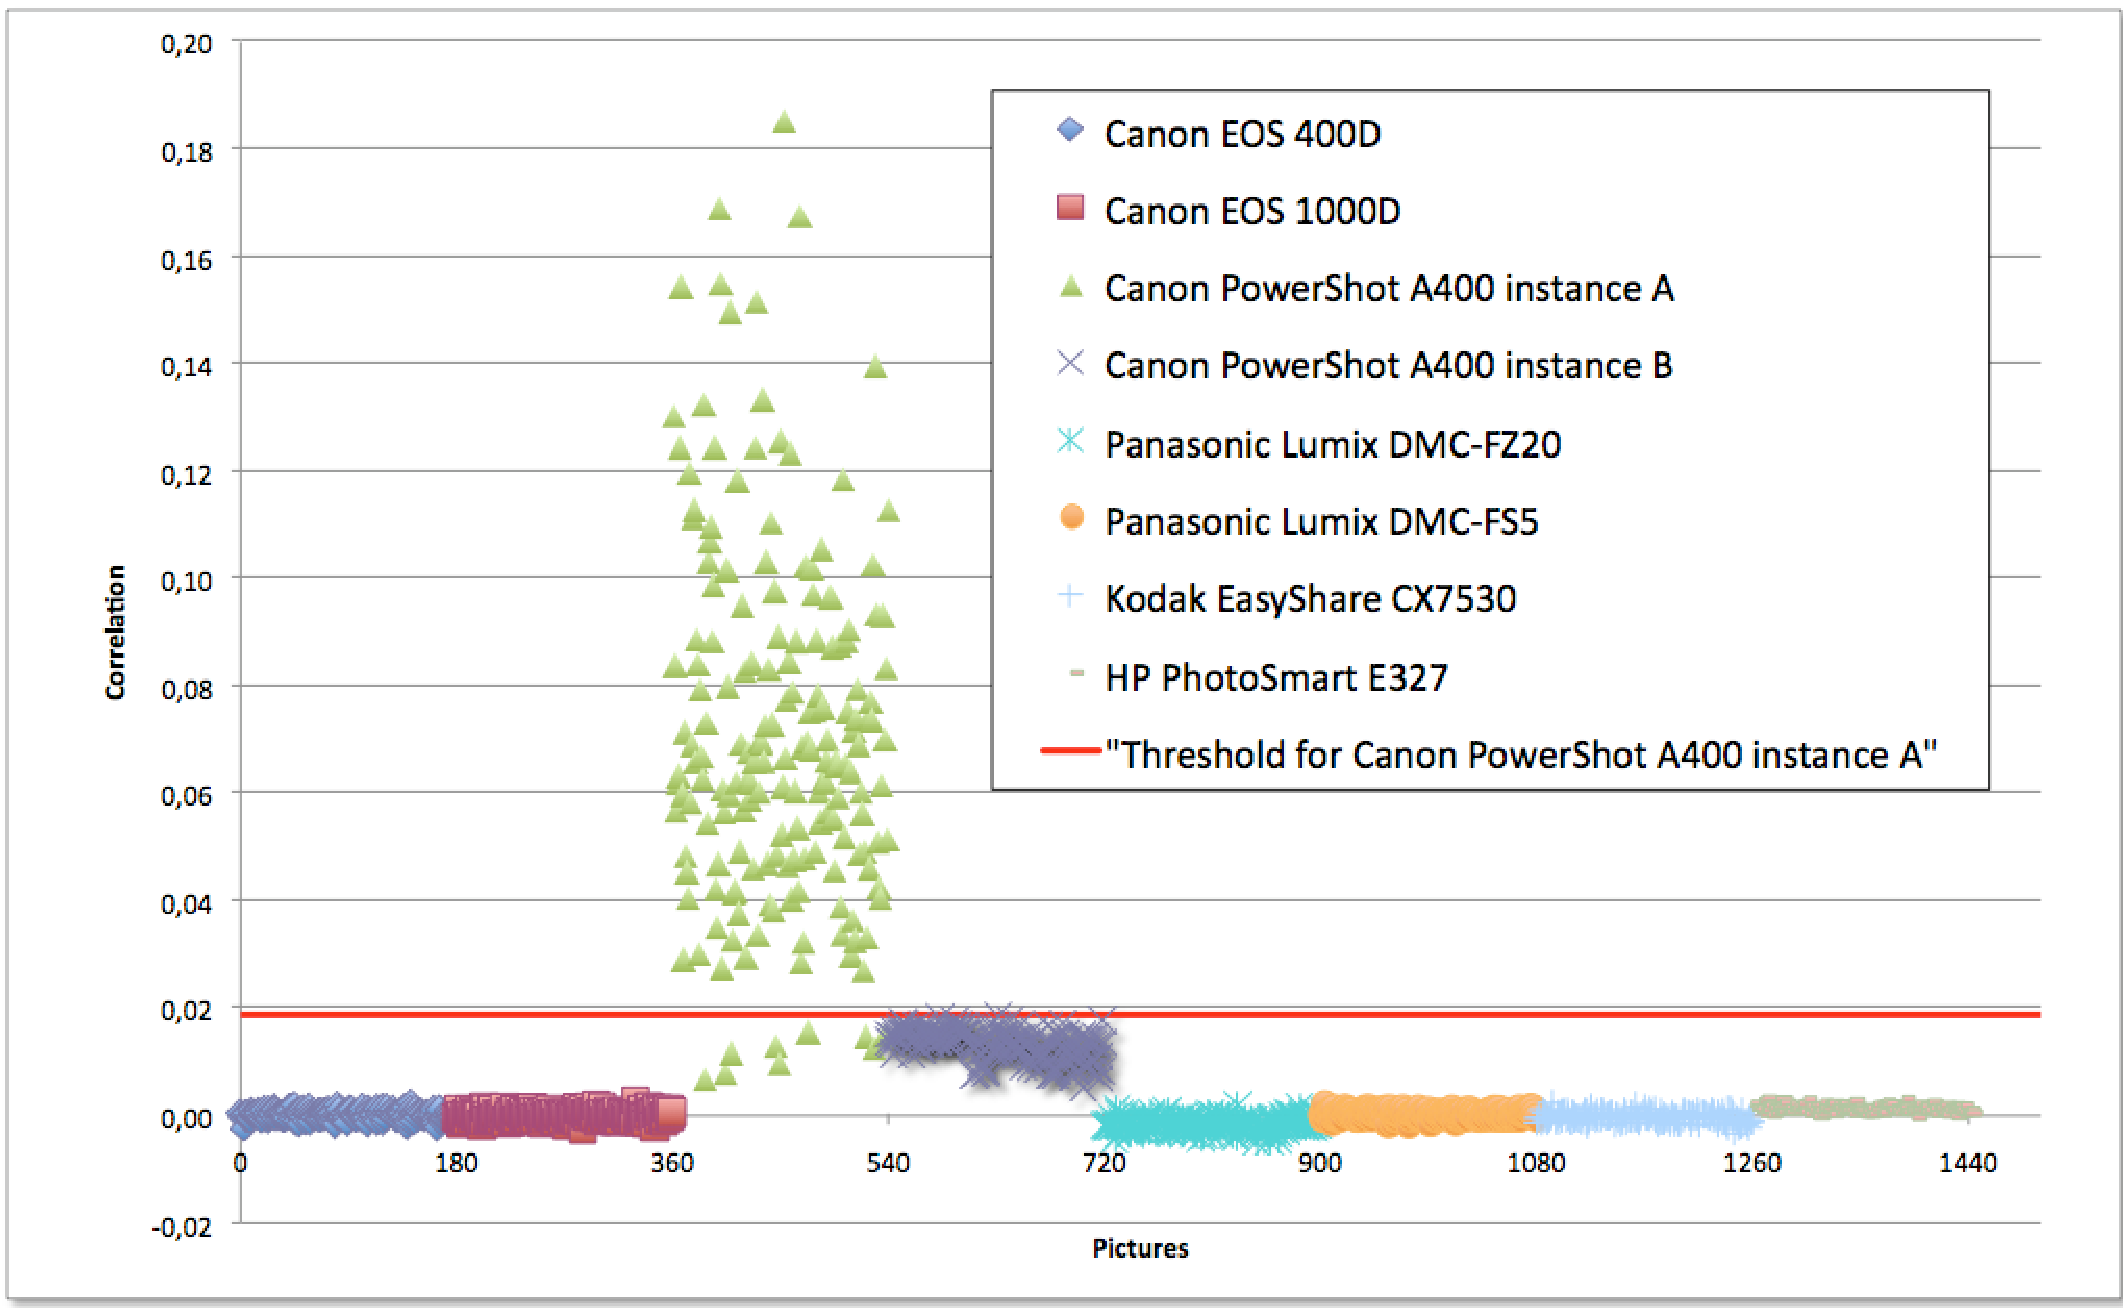
\includegraphics[width=17.4truecm]{A400_180Color.pdf}}
%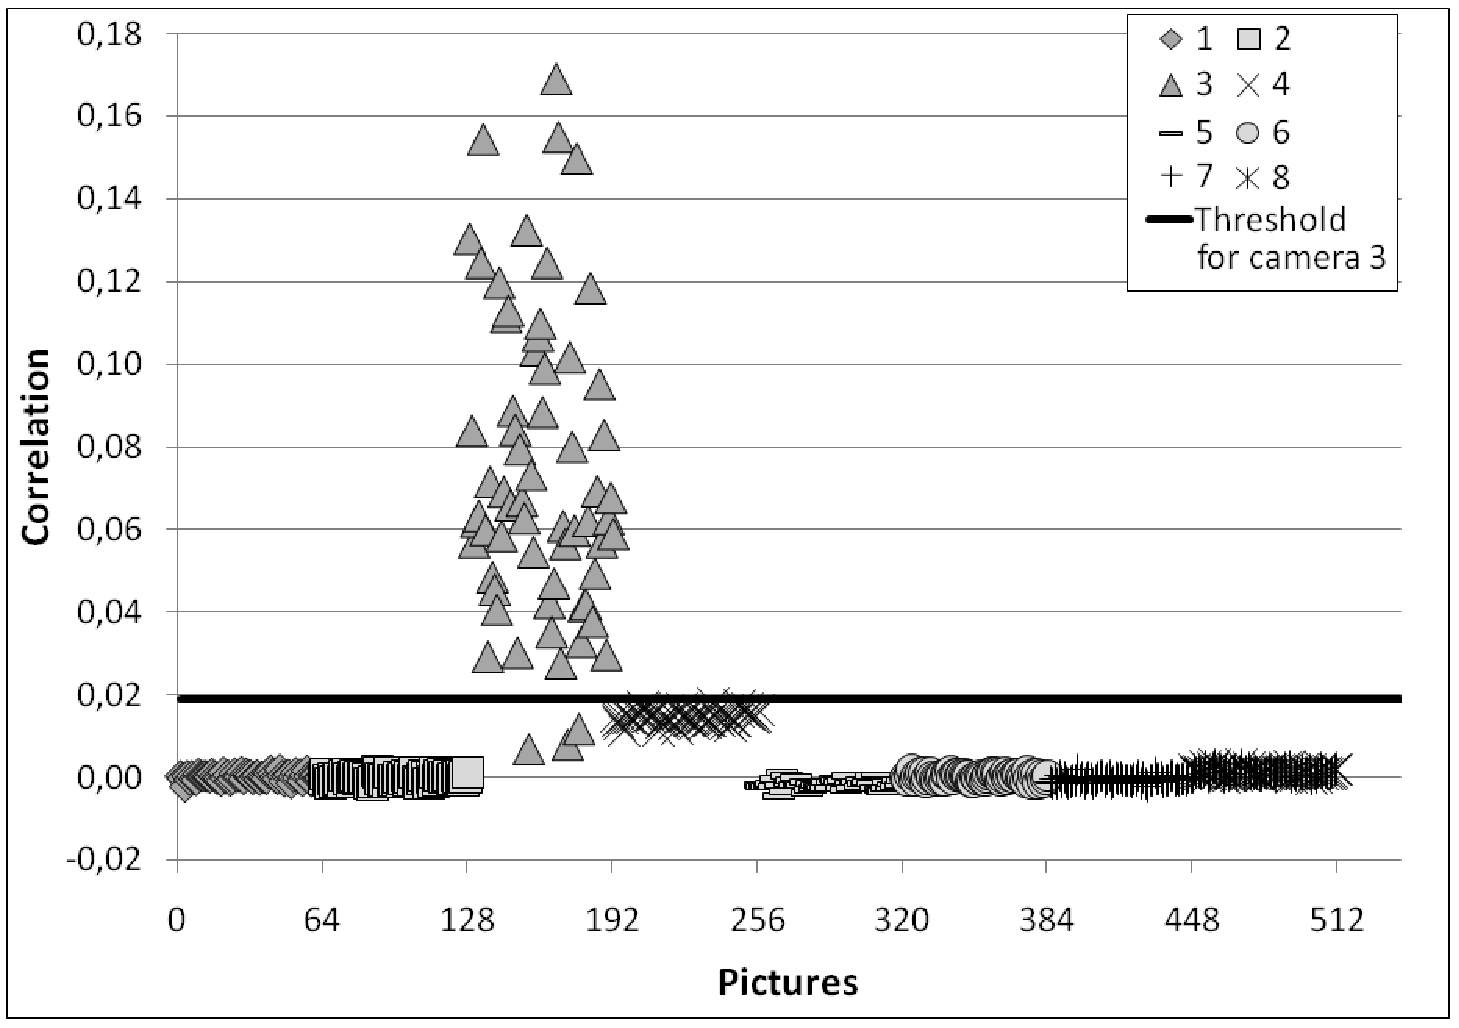
\includegraphics[width=12truecm]{A400_64Gray.pdf}}
\caption{Scatter plot of the correlations between all the images of the data set and the Image Reference Pattern of the camera with ID 3.}
\label{scatterPlot}
\end{figure*}
For each camera model $c \in C=\{1, 2, \dots, 8\}$ two sets of images were collected: the {\em Images for Reference Pattern} (IRP) and the {\em Images for Testing} (IT). IRP$_{c}$ / IT$_{c}$ denotes the IRP / IT sets for the camera $c$. The IRP$_{c}$ set is composed of 128 images collected by taking pictures of a uniform white surface. The images were taken on a tripod, with no flash, auto-focus, no-zoom, best JPEG compression quality, and with all the other options set to their default values. The IT$_{c}$ set is made up of 180 images portraying different types of subjects. In this case, the images were taken using different types of settings, with the exception of the JPEG compression quality as well as the image size, which were always set to maximum. 

% Le formule che seguivano non mi pare aggiungessero qualcosa a quanto gi� detto. Nemmeno facciamo pi� uso di questa notazione nel resto del paper, e quindi possiamo evitare di definire tutte queste cose e sfruttare lo spazio che si libera per ingrandire una delle due figure.
%
%\[C=\{ID01, ID02, \dots, ID02\}\]
%\[\forall c \in C, ~~~~~~~ \left | IT_{c} \right | = 64, ~~~~~~~ \left | IRP_{c} \right | = 64\]\\
%
%The dataset of the image for testing IT is $D_{IT}$ which can be formalized as: \[D_{IT} = \bigcup_{c \in C} IT_{c}\] resulting in:
%
%\[\left | D_{IT} \right | = \sum_{c \in C} \left | IT_{c} \right |  = \left | C \right | * \left | IT_{c} \right | = 8 * 64 = 512\]
%
%while the dataset of the image reference pattern (IRP) is $D_{IRP}$ and can be formalized as: \[D_{IRP} = \bigcup_{c \in C} IRP_{c}\] resulting in:
%
%\[\left | D_{IRP} \right | = \sum_{c \in C} \left | IRP_{c} \right |  = \left | C \right | * \left | IRP_{c} \right | = 8 * 128 = 1024\]

%%%\[ IRP_{total}=\sum_{c \in C} \left | IRP_{c} \right |   ~~~C \in \{ID01, ID02, \dots, ID08\} \]
%%%
%%%resulting in \[ \left | IRP_{c} \right | * \left | C \right | = 128 * 8 = 1024 \]
%%%
%%%\[ IT_{total}=\sum_{c \in C} \left | IT_{c} \right |   ~~~~~~~C \in \{ID01, ID02, \dots, ID08\}  \]
%%%
%%%resulting in \[ \left | IT_{c} \right | * \left | C \right | = 64 * 8 = 512 \]
The effectiveness of the identification was measured by counting the number of pictures erroneously rejected by the identification technique over the total number of pictures taken with a certain camera (FRR). Moreover, in all the tests, the decision thresholds were set in such a way to keep to $0$ the total number of pictures erroneously classified as taken with a certain camera (FAR). 


%All the tests were run on a server equipped with two 4-core Intel Xeon X7350 processors at 2.93GHz and using the Linux Ubuntu operating system.
%In order to see the effectiveness of the implemented method, we conducted several experiments.
%After we found that the method works well, we have tested it on various operators to check the goodness.
%We chose the dataset of images and all tests were performed on this set. In the presentation of results,
% in addition to the value of FRR was also indicated the number of images not recognized. 
% This indicator allows us an immediate reading and comparing data.
%In this section we describe first the cameras used and the way we followed to create the image sets. 
%Secondly what kind of experiments we performed in.


\begin{table*}[bht]
\centering
\caption{Decision thresholds, FRR and number of images rejected on the red channel for the tests Sub, Crop and Resize.}

 \begin{tabular}{  | c  | c  |c  | c  | c  | c  | c  | c  |c  | c  |} 

\hline

& \multicolumn{3}{|c|}{ \textbf{Sub} } & \multicolumn{3}{|c|}{ \textbf{Crop} }  & \multicolumn{3}{|c|}{ \textbf{Resize} }\\ \hline
%{\textbf{ID}}& Decision threshold & Images rejected (FRR) & Decision threshold& Images rejected (FRR) & Decision threshold& Images rejected (FRR)  \\ \hline

\multirow{2}{*} {\textbf{ID}}& Decision & Images & FRR & Decision & Images  & FRR & Decision & Images & FRR  \\ 
& threshold & rejected & & threshold & rejected &   & threshold & rejected &   \\ 

\hline

%\begin{tabular}{  | c   | p{1.8cm} | p{1.8cm}  |  p{1.8cm} | p{1.8cm}  | p{1.8cm} | p{1.8cm}  |} 
%\hline
%& \multicolumn{2}{|c|}{ \textbf{Sub} } & \multicolumn{2}{|c|}{ \textbf{Crop} }  & \multicolumn{2}{|c|}{ \textbf{Resize} }\\ \hline
%{\textbf{ID}}& Decision threshold& Images rejected (FRR) & Decision threshold& Images rejected (FRR) & Decision threshold& Images rejected (FRR)  \\ \hline

1 &	0,021 	& 	20 & 0,111	& 0,008 	& |& |			&	0,008	&	| & |\\
2 &	0,021 	& 	29 & 0,161	& 0,007 	& |& |			&	0,007	&	|& | \\ 
3 &	0,024  	& 	18 &0,1 	& 0,018	& 9 &0,05	&	0,018	&	9 &0,05 \\ 
4 &	0,024  	& 	6 &0,033 	& 0,025	& |& |			&	0,025 	&	| & |\\ 
5 &   0,052  	&	1 &0,005		& 0,046 	& 1 &0,005	& 	0,035 	&	|& | \\
6 &	0,026  	&	5 &0,027		& 0,018	 & |& |			&	0,018 	&	|& | \\ 
7 &	0,013 	&	156 &0,866	& 0,003	& 138 &0,766	&	0,003	&	2 &0,011 \\
8 &	0,037  	&	5 &0,027		& 0,022	& 3 & 0,016	&	0,014 	&	| & |\\ \hline 
%\hline
%\multicolumn{2}{|c|}{total number of images rejected} & 240 & & 151 & & 11 \\
%\hline
\end{tabular}
\label{db8SubCropResize}
\end{table*}



\section{Experimental Analysis}
\label{sec:exp_ana}
All the following tests have been conducted on a data set composed of images that have been knowingly
modified in order to test the effectiveness of the identification tecnique by \Lukas.\

\subsection{Test 1}\label{exp1}


% We present and discuss the results of the experiments conducted on the image
% set using our implementation of the tecnique proposed by Lukas {\em
%   et al}, using the following experiments:
% \begin{itemize}
% \item{}images matching the camera fingerprint.
% \item{}Error rates computed from the FAR and FRR.
% \end{itemize}

A preliminary problem to be faced when applying the method by Luk{\' a\v s} {\em et  al.} is to ensure that the two images to be correlated (i.e., the image reference pattern and the image to be identified) have the same size. This condition can be easily met in three different ways:

\begin{itemize}
\item{} Extract from both images two sub-images of the same size ({\bf Sub}). In our case, extract two images originating at point $(0,0)$ and having size 512x512;
\item{} Crop the larger image to match the smaller image ({\bf Crop});
\item{} Resize the larger image to match the smaller image ({\bf Resize}).
\end{itemize}

The original method proposed by~\Lukas\ uses the {\bf Crop} approach. In this study, it was decided to also test the other two approaches in order to determine which one performs better. According to the tests, presented in Table~\ref{db8SubCropResize},  the best approach seems to be {\bf Resize} while the worst is {\bf Sub}. The reason for such a bad performance is likely to be due to the elimination of a large part of the original image, when processing large pictures. The average resolution of the pictures used in the tests is near 2560x1920. As a consequence of this, the cropped image, whose size is fixed to 512x512, retains only the 5\% of the original image as well as its signature, and thus is subject to a worse correlation. In all the remaining tests presented in this paper, when needed, the {\bf Resize} technique will be used.
%
%For each of the points above we performed an experiment, naming 
%respectively {\em EX1-512x512}, {\em EX2-Crop} and {\em EX3-Resize}, to see which 
%of the three approaches was the best.
%
%In the method presented by Lukas {\em et al.}, to calculate the correlation, 
%they cropped the biggest image to the smallest. 
%
%
%
%Our experimental results show that using 
%the resizing of the biggest image to the tiny image get better score.
%Indeed, as can be seen in Table \ref{db8Resize}, the total number of images not recognized 
%in the experiment {\em EX3-Resize} are {XXX} fewer than the number of images  not 
%recognized in the experiment {\em EX2-Crop} (see \ref{db8Crop}).

Figure~\ref{scatterPlot} presents the scatter plot of the correlations between all the images of the data set 
and the image reference pattern (IRP) of the Canon PowerShot A400 instance A (the camera with ID 3). It is interesting to note that this camera model is present twice in the experiments (instance A and instance B). The majority of the correlations between the IRP and images taken using camera with ID 3 is considerably above the decision thresholds, thus leading to a correct classifications. Pictures taken using different camera models exhibit a very small correlation value, close to zero. Finally, picture taken using camera with ID 4 (i.e., same camera model, different instance) feature higher correlation values which are, anyway, under the decision thresholds. 

\begin{table*}[hbt]
\centering
\caption{Decision thresholds, FRR and number of images rejected on the red channel for the tests ALA, ACS and ACO.}
%\begin{tabular}{  | c  | p{1.8cm}  | p{1.8cm}  | p{1.8cm}  |  p{1.8cm} | p{1.8cm}  | p{1.8cm} | p{1.8cm}  |} 
% dimensioni tabella riformattata
% \begin{tabular}{  | c  | c  | p{1.1cm}  | p{1.0cm}  |  p{1.3cm} | p{1.1cm}  | p{1.0cm} | p{1.3cm}  | p{1.1cm} | p{1.0cm}|} 
 \begin{tabular}{  | c  | c  |c  | c  | c  | c  | c  | c  |c  | c  |} 

\hline

& \multicolumn{3}{|c|}{ \textbf{ALA} } & \multicolumn{3}{|c|}{ \textbf{ACS} }  & \multicolumn{3}{|c|}{ \textbf{ACO} }\\ \hline
%{\textbf{ID}}& Decision threshold & Images rejected (FRR) & Decision threshold& Images rejected (FRR) & Decision threshold& Images rejected (FRR)  \\ \hline

\multirow{2}{*} {\textbf{ID}}& Decision & Images & FRR & Decision & Images  & FRR & Decision & Images & FRR  \\ 
& threshold & rejected & & threshold & rejected &   & threshold & rejected &   \\ 


\hline

1 &	0,008	& 	|& 	|			& 0,008			& |& 	|			&	0,009		   	&		|& 	|	 \\
2 &	0,004 	& 	2 & 0,011		& 0,004			& 2 & 0,011&	0,005		   	&		2 &0,011	 \\ 
3 &	0,022  	& 	11 & 0,061	& 0,019			& 11 & 0,061	&	0,019			&		11 & 0,061  \\ 
4 &	0,019  	& 	2 &0,011 	& 0,02		& 2 & 0,011	&	0,02			&		2 & 0,011 	\\ 
5 & 	0,035  	&	| &	|			& 0,035			& |&	|			& 	0,0352			& 		|  &	|\\
6 &	0,001  	&	7 &0,038 	& 0,003			& 7 &0,039	&	0,0019			&		7 &0,039 \\ 
7 &	0,003  	&	2 &0,011		& 0,003			& 2 &0,011	&	0,003			&		2 &0,011 \\
8 &	0,014  	&	| &	|			& 0,014			& |&	|			&	0,014			&		|	&	| \\ \hline 
%\hline
%\multicolumn{2}{|c|}{total number of images rejected} & 24 & & 24 & & 24 \\
%\hline
\end{tabular}
\label{db8AutoEXP}
\end{table*}



\subsection{Test 2}\label{exp2}

The second test was intended to assess the resilience of the method by~\Lukas\ when used for classifying pictures that have been subjected to some sort of pre-processing. The test was organized by first applying six different commonly-used image processing operations to the data set used in the previous test. Then, the identification method on the resulting data sets was applied, using, for each camera, the same reference pattern and decision threshold established in the previous test. Finally, the resulting classification was compared with the results of the classification on the original (i.e., not pre-processed) pictures. The operations that were considered in the tests, as implemented by the Adobe Photoshop software~\cite{PhotoshopSITE}, are:

\begin{itemize}
\item{\bf Auto Level Adjustment} ({\bf \sl ALA}):  this function automatically corrects the highlights and shadows in a picture and adjusts the tones so that the lowest level in the picture is completely black and the brightest white is full white. Auto Levels tunes each color channel individually, and this may remove or introduce color casts;
\item{\bf Auto Contrast} ({\bf \sl ACS}): this function adjusts the overall contrast and mixture of colors in an image, without introducing or removing color casts,
and permits to create a more accurate tonal and color-correction;
\item{\bf Auto Color} ({\bf \sl ACO}): this function adjusts contrast and color of an image by neutralizing the midtones and clipping the white and black pixels;
\item{\bf Resizing} ({\bf \sl R75}, {\bf \sl R50}, {\bf \sl R25}): this operation rescales the image to match a smaller size; the interpolation algorithm is \emph{bi-cubic} which produces noticeably sharper images than other methods such as \emph{bilinear} or \emph{nearest neighbour}, and it is a good balance between processing time and output quality. The images were processed with this operation by changing the scale factor. Pictures with the image size of 75\%, 50\% and 25\%  of its original sizes were obtained.
\end{itemize}


\begin{table}[b]
\centering
\caption{Number of images rejected on manipulating pictures with thresholds computed as in Test 1 (Resize).}
\begin{tabular}{  |c  | c | c |  c | c  | c | c  |  c  |} 
\hline
& \multicolumn{7}{|c|}{ \textbf{Operation}} \\ \hline
{\textbf{ID}}& \textbf{No} & \textbf{ALA} & \textbf{ACS} & \textbf{ACO} & \textbf{R75} & \textbf{R50} & \textbf{R25} \\ \hline
1 		& | 	& | 	& | 	& | 	& | 	& | 	& 2 \\
2 		& | 	& 4	& 4 	& 3 	& 2 	& 2 	& 14 \\
3 		& 9 	& 11 	& 11 	& 11 	& 11 	& 15 	& 49 \\
4 		& | 	& 3 	& 3 	& 3 	& 3 	& 7 	&  51 \\
5 		& | 	& 1 	& 1 	& 1	& | 	& 1	& 108 \\
6 		& | 	& 7 	& 7 	& 7 	& 10 	& 12 	& 97 \\
7 		& 2	& 2 	& 2 	& 2 	& 2 	& 2 	& 2 \\
8 		& | 	& 1 	& 1 	& 1 	& 2 	& 2 	& 40 \\ \hline
 \hline
{Tot.} 	& 11	& 29 	& 29	& 28 	& 30	& 41 	& 363 \\
\hline
\end{tabular}
\label{tableExp2}
\end{table}


The results of these tests, presented in Table~\ref{tableExp2}, are noteworthy. A small increase in the number of erroneously rejected images can be observed when considering the pictures processed with the ALA, ACS and ACO operations. This increase is much more significant when considering the resized images. Here, the number of rejected images is high and grows linearly with the resize factor. By examining in details these results, it is worth noting that there are some camera models where the identification method performs very poorly when used with resized images. It is the case of models $3$, $4$, $6$, and, especially, model $5$. This seems to suggest either that the resize operation may have a very strong influence on the correlation between the picture and the reference pattern noise, and that this influence may vary greatly according to the camera being used, even for different cameras of the same model. Moreover, it can ben noted that if the decision thresholds are chosen using, as a reference, pictures that have not been previously pre-processed, the identification method may likely fail. 

%Il secondo esperimento � consistito in 6 test che condividevano lo stesso data set $D_{IT}$ su cui
%sono stati applicati diversi ``operatori''. Per ``operatore'' intendiamo un'operazione di editing 
%effettuata sull'immagine atta a modificarne alcune caratteristiche peculiari. 
%Gli operatori utilizzati forniti dal software Adobe Photoshop \cite{PhotoshopSITE} sono:
%
%
%Tutti gli operatori tranne il {\bf Resizing} non sono in alcun modo parametrizzabili e quindi
%sono stati utilizzati ``as-is''. Per il {\bf Resizing} abbiamo sottoposto il data set a tre differenti
%ridimensionamenti, rispettivamente del 75\%, del 50\% e del 25\% rispetto alla taglia originale
%di ogni foto.
%Il risultato dell'applicazione di ogni operatore (ALA, ACS, ACO, R75, R50 and R25) ha creato
%un nuovo data set sul quale � stato applicato il metodo di Luk{\' a\v s} {\em et  al.} utilizzando
%la tecnica del {\bf Resize} come mostrato nell'esperimento 1 (see subsection~\ref{exp1}).
%-----------------------------------------------------------------------------------------------


\begin{table*}[htb]
\centering
\caption{Decision thresholds, FRR and number of images rejected on the red channel for the tests R75, R50 and R25.}


 \begin{tabular}{  | c  | c  |c  | c  | c  | c  | c  | c  |c  | c  |} 

\hline

& \multicolumn{3}{|c|}{ \textbf{R75} } & \multicolumn{3}{|c|}{ \textbf{R50} }  & \multicolumn{3}{|c|}{ \textbf{R25} }\\ \hline
%{\textbf{ID}}& Decision threshold & Images rejected (FRR) & Decision threshold& Images rejected (FRR) & Decision threshold& Images rejected (FRR)  \\ \hline

\multirow{2}{*} {\textbf{ID}}& Decision & Images & FRR & Decision & Images  & FRR & Decision & Images & FRR  \\ 
& threshold & rejected & & threshold & rejected &   & threshold & rejected &   \\ 


\hline


%\begin{tabular}{  | c   | p{1.8cm} | p{1.8cm}  |  p{1.8cm} | p{1.8cm}  | p{1.8cm} | p{1.8cm}  |} 
%\hline
%& \multicolumn{2}{|c|}{ \textbf{R75} } & \multicolumn{2}{|c|}{ \textbf{R50} }  & \multicolumn{2}{|c|}{ \textbf{R25} }\\ \hline
%{\textbf{ID}}& Decision threshold& Images rejected (FRR) & Decision threshold& Images rejected (FRR) & Decision threshold& Images rejected (FRR)  \\ \hline

1 &	0,011	& 	|& 	|& 0,01 & |	& |	&	0,009		   	&	2 & 0,011	 \\
2 &	0,004	& 	2 &0,011		& -0,001 & |& |			&	0,0067		   	&	9 &0,05	 \\ 
3 &	0,011	& 	11 &0,061	& -0,002 & |	& |		&	0,009			&	11 &0,061  \\ 
4 &	0,013 	& 	2 &0,011 	& 0,009 & 2 &0,0111	&	0,007		&2 &0,011 	\\ 
5 & 	0,037  	&	|& |			& 0,033 & |	& |		& 	0,017& 		| & | \\
6 &	0,002  	&	7 &0,039 	& 0,003 & 7 &0,0389	&	0,005		&13 &0,072 \\ 
7 &	0,004  	&	2 &0,011		& 0,006 & 2 &0,0111	&	0,009&		2 &0,011 \\
8 &	0,013  	&	|& |			& 0,009 & |& |			&	0,007&		5 &0,028	 \\ \hline 
%\hline\hline \hline
%\multicolumn{2}{|c|}{total number of images rejected} & 24 & & 11 & & 44 \\
%\hline
\end{tabular}
\label{resize75_50_25}
\end{table*}




\subsection{Test 3}\label{exp3}
In the previous test, it can be observed that when trying to classify pre-processed pictures using a classifier that has been tuned for unmodified pictures, the identification method by~\Lukas\ may fail, in some cases, with a very high probability. These failures are mostly due to the alteration of the pattern noise existing in a processed picture. This alteration implies a smaller correlation with the reference pattern noise. A natural solution to this problem consists in lowering the decision threshold used during the classification, so as to also correctly identify pictures with smaller correlations. 

This is what has been done with Test 3. The results, documented in Table~\ref{db8AutoEXP}, show a significant improvement in the quality of the classification, with respect to the previous test. In this case, it has been possible to obtain FRR rates which are very similar to those experienced with the first test. However, such a result comes at a cost. The new decision thresholds are, in some cases, much lower than the original ones. For example, the decision threshold relating to camera $5$ had to be lowered to more than $90\%$ of its original value, thus raising the possibility of wrong classifications on larger data sets. So, this approach should be generally avoided as it tends to increase the FAR as well as the FRR. 

The same behaviour can be noted when using the R75, R50, and R25 operations. As shown in Table~\ref{resize75_50_25}, even for these operations, the thresholds change without any correlation with the percentage of resize. In other words, what should have been expected with this test is that reducing the image size would decrease the correlation index. This happens only in some cases like for example in the case with camera ID 8.
%In practice this does not happen for all the cameras with different behaviour for some cameras. In particular, the threshold of the camera with ID 8 decreases while those for camera with ID 7 increases.


\section{OSNs and OPSs Experimentations}\label{exp4}
All the previous tests have been conducted on unmodified pictures or on pictures that have been intentionally modified by the end-user, using  photo-editing tools. In the real world, it is quite usual to upload digital pictures on OPSs or OSNs websites, without any prior modification. This could lead to the wrong conclusion that the pictures found on these sites retain the same properties of their original counterparts and, so, that can be used for the digital identification process.  Instead, OSNs and OPSs websites usually process uploaded pictures in order to reduce their size and to speed-up their handling. The arising question is: does this pre-processings puts at risk the effectiveness of  the~\Lukas\ identification technique when applied to pictures retrieved from one of these sites?

\subsection{Test 4}
This test was aimed at determining which OSNs and OPSs modify pictures uploaded by users. This has been done, first of all, by choosing a set of OSNs and OPSs according to their popularity. Then, several sets of pictures have been uploaded and downloaded  from all these sites. The downloaded pictures have been analyzed in order to understand if, and how, they have been modified.

In Table~\ref{photo_sharing_statistics} the results of one of these experiments, carried out with a sample picture of $3.888$x$2.592$ pixels and size of $2.275$ kilobytes, are presented. For each site, it has been checked if the picture was modified or not and, in the former case, it has been measured the size and the resolution of the modified picture.

These experiments show that only the following OSNs and OPSs, among the considered ones, process and modify uploaded pictures.

\begin{table}[htb]
\centering

\caption{Modifications performed by several OSN / OPS sites on a target image of resolution $3.888$x$2.592$ pixels and size $2.275$ kilobytes.}

\begin{tabular}{  |l | c | c  |  c |} 
%\begin{tabular}{  |l | c | m{1.7cm}  | m{1.7cm} |} 

\hline

Site & Modified & New resolution & New size \\ \hline

Facebook & Yes & $720$x$480$ & $53$ Kb  \\
Flickr & No & $3.888$x$2.592$ & $2.275$ Kb \\
MySpace & Yes  & $600$x$399$ & $33$ Kb\\
PhotoBucket & Yes  & $1.023$x$682$ & $131$ Kb \\
Picasa & No & $3.888$x$2.592$ & $2.275$ Kb\\
Twitpic & No & $3.888$x$2.592$ & $2.275$ Kb  \\

\hline
\end{tabular}
\label{photo_sharing_statistics}
\end{table}


\paragraph{Facebook} (FAC) is currently the most used OSN in the world, with more than $500$ million active users. It offers a relatively simple support for uploading and sharing photos. No limit is apparently put on the size of the pictures that can be uploaded. 

Currently, service administrators do not disclose any information about the way images are processed and stored on their servers. However the experiments revealed a strong compression, via downsampling, of all the pictures uploaded with a standard resolution of $720$ pixels on the long edge. This is evidently done in order to cope with the huge amount of pictures uploaded daily. 

Recently, service administrators have announced an upgrade on the maximum size of the images stored in the Facebook database. According to this new setting, it will be possible to upload also high-resolution images, with a maximum size of $2.048$ pixels on the long edge. 

\paragraph{Photobucket} (PHB) is one of the most popular OPS with a massive audience of more than $23$ million monthly unique users in the U.S., and over four million images uploaded per day from the web and smartphones~\cite{PhotoBucketStat}. Photobucket offers a simple support for uploading and dowloading and sharing photos. Like in the Facebook case, no information is disclosed about the way pictures are stored on their servers. However, the experiments revealed a compression process, albeit less aggressive than the one used by Facebook. 

%In our experiments the images was published on Photobucket and later the images was downloaded. These images constitutes the set PHB of images where test the method of Lukas.

% figura indicante la variazione della soglia 
 \begin{figure*}[bth]
 \centerline{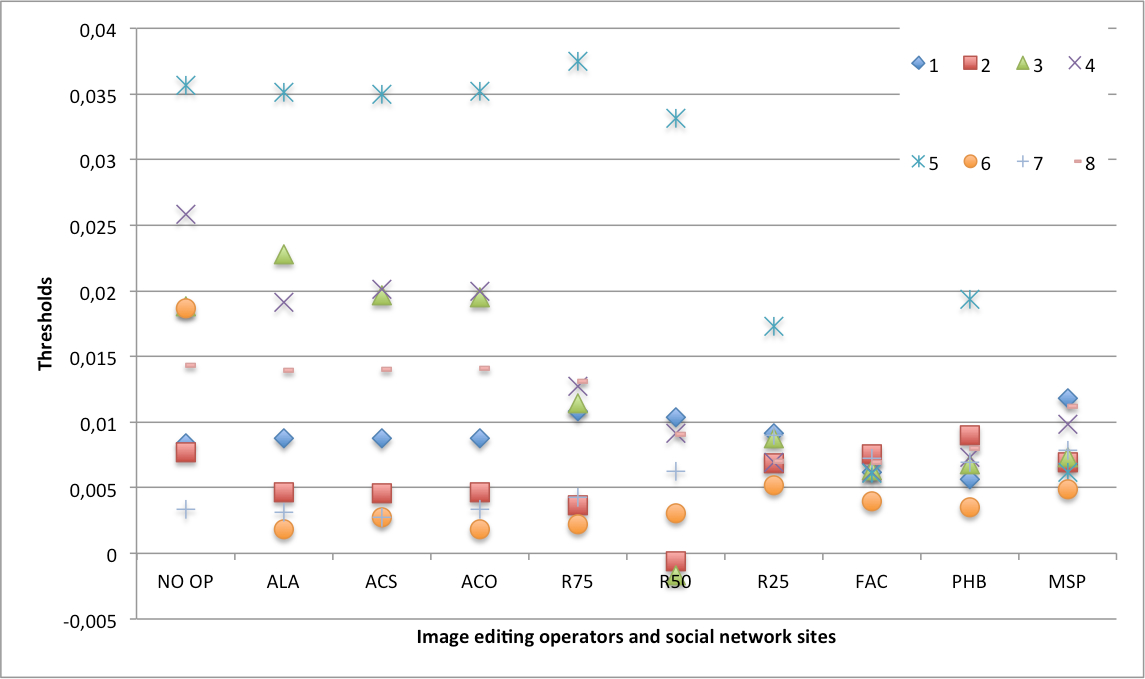
\includegraphics[width=17.4truecm]{ThresholdColor180.pdf}}
% \centerline{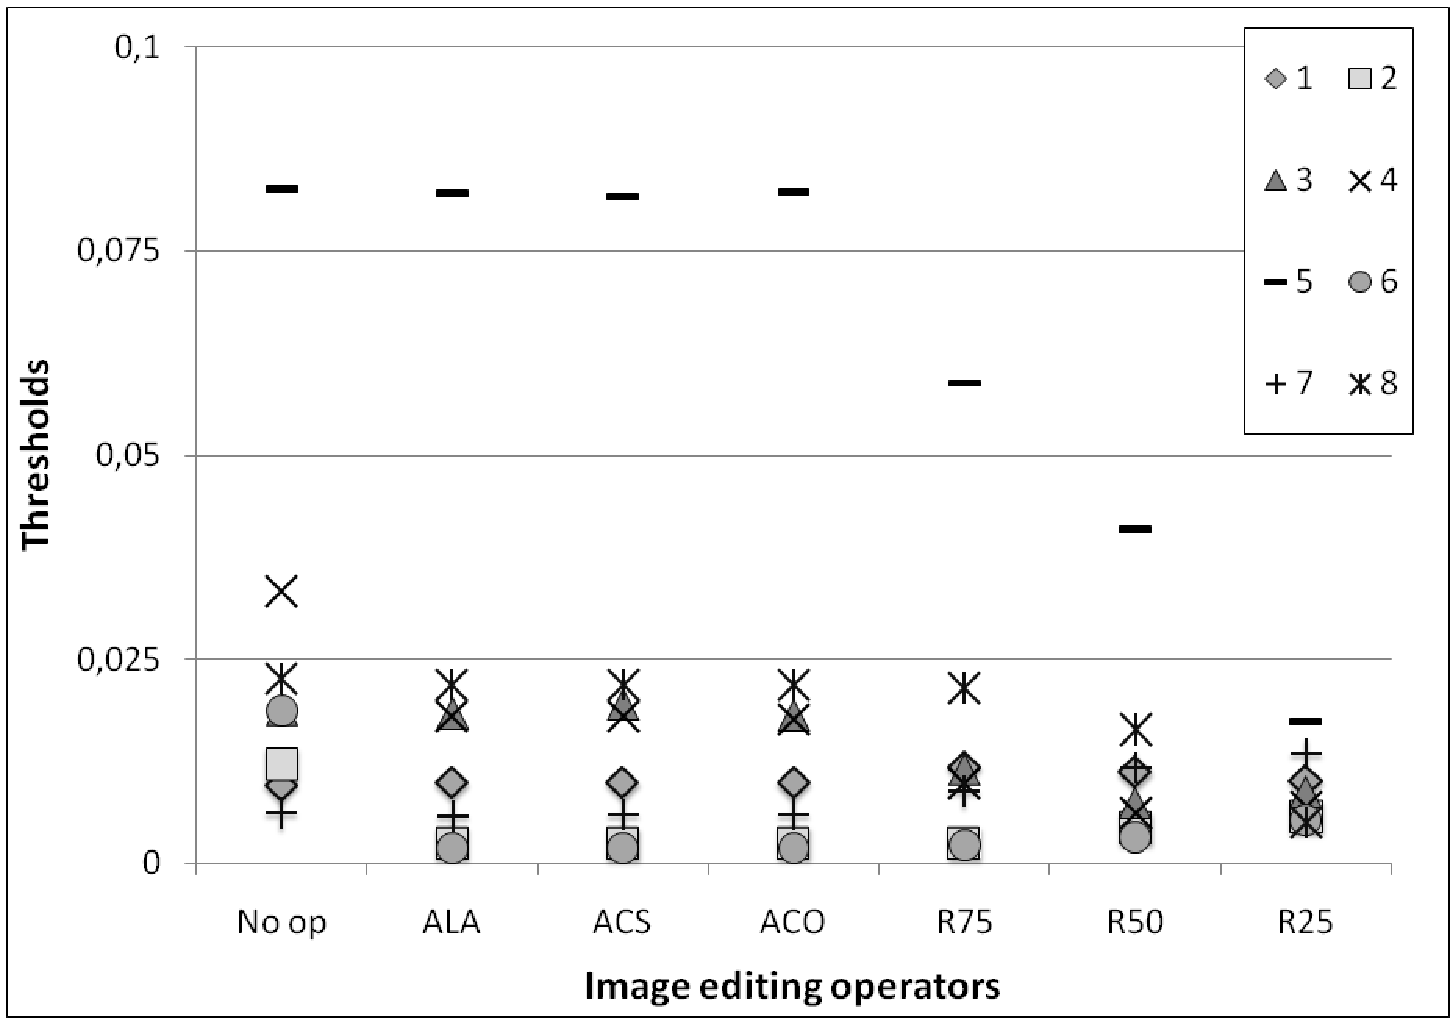
\includegraphics[width=10truecm]{ThresholdGray.pdf}}
 \caption{Thresholds values used according to the pre-processing operations being tested.}
 \label{thresholdsChart}
 \end{figure*}
%


\paragraph{MySpace} (MSP) is a OSN where users can share music, videos and pictures. No limit is put on the number and on the size of the uploadable pictures. However, even in this case, the experiments revealed a strong compression of the uploaded images, both in terms of size and downsampling. 

%In our experiments the images was published on MySpace and later the images was downloaded. These images constitutes the set MSP of images where test the method of Lukas.

\begin{table}[bht]
\centering
\caption{Number of images rejected on pictures previously uploaded on a OSN / OPS with thresholds computed as in Test 1 (Resize).}
\begin{tabular}{  |c  | c | c |  c | c   |} 
\hline
& \multicolumn{4}{|c|}{ \textbf{OSN / OPS service}} \\ \hline
{\textbf{ID}}& \textbf{No} & \textbf{FAC} & \textbf{PHB} & \textbf{MSP} \\ \hline
1 		& | 	& 178 	& 96 		& 180	 \\
2 		& | 	& 176	& 80 		& 180 	 \\
3 		& 9 	& 171 	& 40 		& 180 	 \\
4 		& | 	& 159 	& 46 		& 180 	 \\
5 		& | 	& 180 	& 104 	& 180	 \\
6 		& | 	& 180 	& 178 	& 180 	\\
7 		& 2	& 2 		& 2 		& 20 	 \\
8 		& | 	& 178 	& 22 		& 180 	 \\ \hline \hline
{Tot.} 	& 11	& 1224	& 568	& 1280 	\\
\hline
\end{tabular}
\label{tableExp4}
\end{table}


\begin{table*}[htb]
\centering
\caption{Decision thresholds, FRR and number of images rejected on the red channel for the tests FAC, PHB and MSP.}

 \begin{tabular}{  | c  | c  |c  | c  | c  | c  | c  | c  |c  | c  |} 

\hline

& \multicolumn{3}{|c|}{ \textbf{FAC} } & \multicolumn{3}{|c|}{ \textbf{PHB} }  & \multicolumn{3}{|c|}{ \textbf{MSP} }\\ \hline
%{\textbf{ID}}& Decision threshold & Images rejected (FRR) & Decision threshold& Images rejected (FRR) & Decision threshold& Images rejected (FRR)  \\ \hline

\multirow{2}{*} {\textbf{ID}}& Decision & Images & FRR & Decision & Images  & FRR & Decision & Images & FRR  \\ 
& threshold & rejected & & threshold & rejected &   & threshold & rejected &   \\ 


\hline

%\begin{tabular}{  |c   | p{1.8cm} | p{1.8cm}  |  p{1.8cm} | p{1.8cm}  | p{1.8cm} | p{1.8cm}  |} 
%\hline
%& \multicolumn{2}{|c|}{ \textbf{FAC} } & \multicolumn{2}{|c|}{ \textbf{PHB} }  & \multicolumn{2}{|c|}{ \textbf{MSP} }\\ \hline
%{\textbf{ID}}& Decision threshold& Images rejected (FRR) & Decision threshold& Images rejected (FRR) & Decision threshold& Images rejected (FRR)  \\ \hline

1 &	0,006		& 	165 &0,913	& 0,006			& 36 &0,2		&	0,012		   	&		180 &1	 \\
2 &	0,008		& 	175 &0,967	& 0,009			& 105 &0,583		&	0,007		   	&		179 &0,994	 \\ 
3 &	0,006		& 	18 &0,093	& 0,007			& 11 &0,061		&	0,007			&		152 &0,844  \\ 
4 &	0,006	 	& 	2 &0,0133 	& 0,007			& 2 &0,011		&	0,01			&		168 &0,933 	\\ 
5 & 	0,006 	 	&	14 &0,06	& 0,0193		& |& |				& 	0,006			& 		160 &0,889 \\
6 &	0,004  		&	84 &0,487 	& 0,003			& 10 &0,056		&	0,005			&		179 &0,994 \\ 
7 &	0,007  		&	4 &0,02	& 0,007			& 2 &0,011		&	0,008			&		90 &0,5 \\
8 &	0,007  		&	68 &0,387	& 0,008			& 2 &0,011		&	0,0112			&		180 &1	 \\ \hline 

%\hline\hline \hline
%\multicolumn{2}{|c|}{total number of images rejected} & 530 & & 168 & & 1288 \\
%\hline
\end{tabular}
\label{socialNetworkExp}
\end{table*}


\subsection{Test 5}
In this test, the~\Lukas\ identification technique has been experimented by applying it on pictures previously uploaded on each of these websites. This experimentation has been first conducted by using the same decision threshold computed in Test 1 of the previous section (see~\ref{exp1}). 
The results, presented in Table~\ref{tableExp4}, show a substantial failure of the identification technique. 
On a side, this was expectable because, as already noted in the previous section, thresholds evaluated using unmodified images imply bad performance when classifying modified pictures. 

On the other side, however, it is worth to note that these bad performances are also much worser than the one experienced on resized pictures in Test 2 (see~\ref{exp2}) and Test 3 (see~\ref{exp3}), especially when processing pictures retrieved from FAC and MSP. This seems to suggest that the reason of this behavior is not only the resizing of the processed images but also to other factors such as, for example, compression tricks of the images retrieved from the considered OSNs/OPSs. 


\subsection{Test 6}
In the last test,  the~\Lukas\ identification technique has been experimented again on the same set of pictures of the previous test by using, this time, thresholds computed by means of images stored and retrieved from the considered OSNs/OPSs (a graphical representation of the updated decision thresholds is available in Figure~\ref{thresholdsChart}). The results, shown in Table~\ref{socialNetworkExp}, confirm a strong improvement of the identification technique with respect to the previous experiment when analyzing pictures retrieved from FAC and PHB. This is especially the case of pictures taken using camera with ID 3 and 4. A fair improvement is also evident for pictures taken using cameras with ID 5, 6 and 8. Instead, the identification is mostly uneffective when processing pictures retrieved from MSP. These differences are probably due to the different compression strategies employed by the considered OSNs/OPSs when uploading pictures. MSP is likely to be the service that adopts the most aggressive strategy, as witnessed by results presented in Table~\ref{photo_sharing_statistics}. 

The bad performance of the \Lukas\ identification technique on pictures retrieved from OSNs/OPSs may also be due to other reasons, apart from the image compression. As a matter of fact, it can not be excluded that OSNs/OPSs may add some kind of ``watermarking'' to all the photos that flow on their websites. Such possibility could have two opposite effects from the Image Forensics point of view. On the one hand, the inscription of a watermark on a picture could alter its inner structure and fool the identification process, thus leading to a wrong classification. On the other hand, if the pictures have been previously ``watermarked'' by the OSNs/OPSs, the eventual ``discovery'' of the adopted watermarking technique could give useful hints in the direction of establishing which is the OSN/OPS service that hosted the image under scrutiny. In this case, what will be assessed is the OSN/OPS that processed the image and not which camera model were adopted to shoot the photo.
%Analyzing Figure~\ref{thresholdsChart}, it can be noted that no relation seem to exists between the thresholds and the manufacturer of the camera models used.
%Moreover, each camera is independent from the others since it presents its own threshold. In fact, the thresholds differ for the same camera model (cameras 3 and 4) and for camera models probably equipped with the same sensor (cameras 1 and 2).
%Furthermore, the figure highlights how the results of the operations are strictly dependent on the camera, showing that the operations do not linearly affect all the cameras.


\section{Conclusions}
\label{sec:conc}

In this paper, the effectiveness of the source camera identification technique from~\Lukas\ has been evaluated, when using, as input, pictures that have been altered by means of commonly used image processing operations. The results of the tests show, first of all, that the classification of the altered images may perform very poorly if the classifier has been tuned using unmodified images (see subsection~\ref{exp2}). A simple solution to this problem is to tune the classifier according to a data set of altered images and, consequently, by lowering the decision thresholds used to establish whether a picture has been taken with a given camera. In this new configuration, the Luk{\' a\v s} method seems to confirm its ability to correctly identify pictures show with a given camera (see subsection~\ref{exp3}), even when processing altered images. However, this solution has an important side-effect, it may increase the false acceptance rate as well. Moreover, there are processing operations, such as resizing and/or increasing the compression factor of a JPEG picture, which seems to have nevertheless a negative effect on the results of the classification. 
As an additional result of the tests, it was noted that the use of a {\em Resize} operation seems to be preferable to a {\em Crop} one when calculating the correlation between two images of different sizes. 

The decrease of the threshold involves, nonetheless, several problems while choosing which one to use 
during a real investigation on a photographic exhibit. In fact, if the threshold computation is performed on a set of ``unaltered'' images, then the obtained threshold  will be greater than the correlation index of a given, altered, image under scrutiny. Otherwise, if the computation of the decision threshold is computed on a set of altered images then the FRR is increased.

The research also investigates if and how OSN/OPS services modify the images that transit on their websites, and tries to establish if the method proposed by \Lukas\ is able to correctly identify images modified in this way. The investigation has been conducted by means of three more tests. The test $4$ determines which OSN/OPS, among a set of them containing some of the most popular ones, alters the pictures. In the test $5$, the \Lukas\ method is applied on photos that have been previously uploaded on the OSNs/OPSs scrutinized in the above step. The results show a significant inadequacy of the identification method when using the same decision threshold computed for the test $1$ (as in subsection~\ref{exp1}). Finally, the test $6$  has been conducted on the same data set of test $2$, but using threshold values pre-computed on images stored and downloaded from the examined OSNs/OPSs. The results validate and confirm the expectations that the identification technique behaves better when using thresholds that have been extracted in the ``correct'' way. Despite this, the identification revealed to be unsuccessful in many cases, mostly because of the compression strategies employed by the considered OSNs/OPSs in order to reduce the size of uploaded images. This problem could be faced by analyzing in details the type of processing applied by the OSN/OPS services on the pictures they host and, consequently, develop {\em ad-hoc} image reference patterns able to cope with these transformations. Another question, worth to be investigated, is whether the other identification techniques would perform better than the one by \Lukas\ or not in such a scenario.

Another factor, that can be further analyzed in a future work, is that the OSNs/OPSs could watermark in some way the images that flow on their websites. The watermarking operations while from one hand could contribute to the bad performance of the \Lukas\ method,  on the other hand could give useful hints in the direction of establishing the OSN/OPS that handled a given photo. In a few words, it would be possible to distinguish if a given photo under investigation has been posted to an OSN/OPS website just analyzing some ``hidden'' characteristics of the photo without relying on its ``evident'' origin.


% use section* for acknowledgment
\begin{acknowledgements}
The authors would like to thank the chief of the CNCPO, V.Q.A.~Dr.~Elvira D'Amato, along with her group, for their valuable suggestions during the research phases.
%The authors would like to thank the members of the CNCPO for their valuable suggestions during the research
Their needs, questions and doubts coming from real and day-by-day investigations have encouraged the
authors to further improve this work. A sincere thanks goes to the group of undergraduates who helped carry out the study.
\end{acknowledgements}



\balance

% BibTeX users please use one of
%\bibliographystyle{spbasic}      % basic style, author-year citations
%\bibliographystyle{spmpsci}      % mathematics and physical sciences
\bibliographystyle{plain}      % mathematics and physical sciences
%\bibliographystyle{spphys}       % APS-like style for physics
\bibliography{SCI_JAIHC}   % name your BibTeX data base

%%%%% Non-BibTeX users please use
%%%%\begin{thebibliography}{}
%%%%%
%%%%% and use \bibitem to create references. Consult the Instructions
%%%%% for authors for reference list style.
%%%%%
%%%%\bibitem{RefJ}
%%%%% Format for Journal Reference
%%%%Author, Article title, Journal, Volume, page numbers (year)
%%%%% Format for books
%%%%\bibitem{RefB}
%%%%Author, Book title, page numbers. Publisher, place (year)
%%%%% etc
%%%%\end{thebibliography}

\end{document}
% end of file template.tex

